\label{chapter:presentProjectState}

\section{Adafruit Bonnet Driver}

The Adafruit 1.3" Color TFT Bonnet for Raspberry Pi \cite{adafruitwebsite} is fully functional on X-HEEP. A BSP (Board Support Package) library has been written to draw images on the display. Added functions include: \\

\begin{itemize}
   \item \textbf{Initialization:} Initialize the display by setting up SPI and GPIO for communication, and sending an initializaiton sequence to configure the display.
   \item \textbf{Write Pixel:} Write a single pixel color at specified X and Y coordinates
   \item \textbf{Fill Screen:} Fill the screen with one specified color.
   \item \textbf{Fill Picture:} Fill the screen with a 120x120 pixel picture provided in a C-array
   \item \textbf{Fill Picture with Shift:} Fill screen with a picture provided in a C-array but with an added shift in X or/and Y coordinates.
   \item \textbf{Manual:} Provided functions to manually set a window and functions and fill it in. This can be used to draw pixels, vertical and horizontal lines, or rectangles.
\end{itemize}

The example program \texttt{example\_adafruit\_bonnet} was created to demonstrate the functionality of the display (see Figure \ref{fig:exampleAdafruitBonnet}). The library, together with the example program provide a framework and guidance for future projects requiring a display. Note that the library, the example program, and the code discussed in the next section are only available in the Github repository \cite{projectRepo} of the project's author. Integration in the official X-HEEP repository \cite{xHeepRepo} is expected.

\begin{figure}[ht]
    \centering
    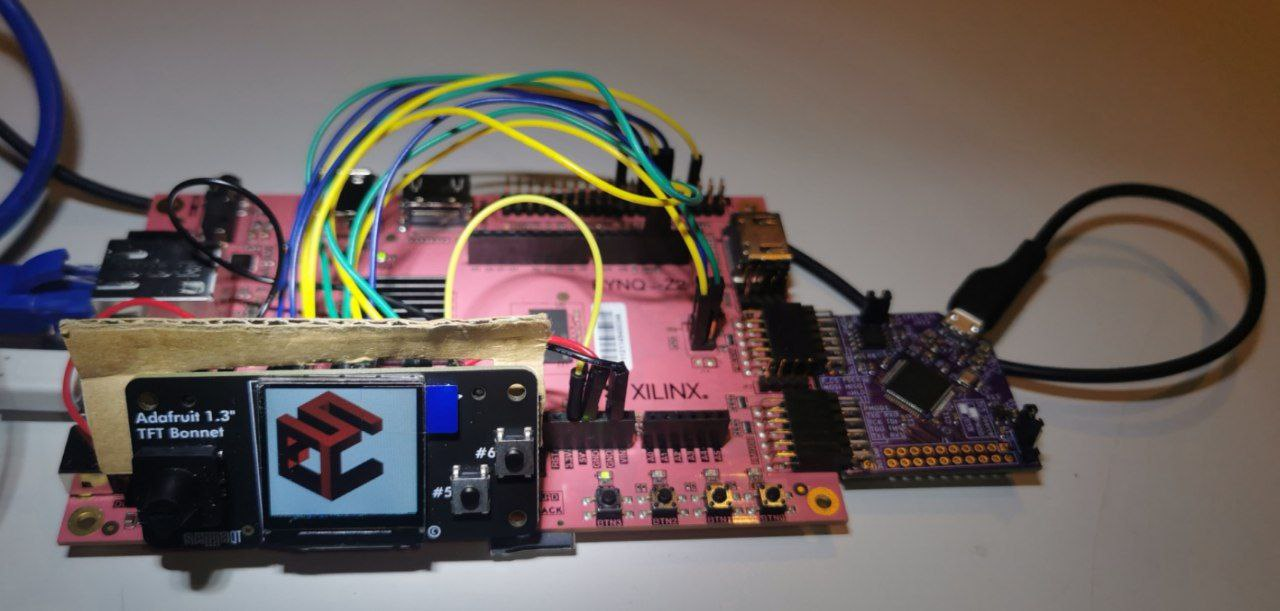
\includegraphics[width=\textwidth]{images/FPGA_ESL_LOGO.jpg}
    \caption{Image of the working \texttt{example\_adafruit\_bonnet} program executed by X-HEEP on FPGA}
    \label{fig:exampleAdafruitBonnet}
\end{figure}


\section{DOOM on X-HEEP}

On June 17, 2024, the DOOM for X-HEEP ran for the first time. Although the display did not show any output, console messages were observed, indicating partial success. Several issues remain unresolved as of today, \today.

\paragraph{\texttt{flash\_load} instead of \texttt{flash\_exec}:} The program compiles for both linker options \texttt{flash\_load} and \texttt{flash\_exec}. The difference between the two is that \texttt{flash\_load} copies the entire program into RAM and then executes operations from RAM. This option is faster but uses more RAM. The \texttt{flash\_exec} option leaves the program in flash and copies one operation at a time to the CPU for execution. This option saves RAM but has worse performance as every signle operation requires a read transaction from the flash. Only the \texttt{flash\_exec} option, however, provides some output when launched. The \texttt{flash\_load} option shows no sign of life. This issue requires further investigation.

\paragraph{SPI Flash Interface:} The interface to get level data from the flash does not seem to work, see comments of Figure \ref{fig:cutecomOutput}. An example program (\texttt{0\_DOOM\_TEST})\cite{projectRepo} has been created to investigate this issue further. One reason could be that DOOM only reacts in \texttt{flash\_exec} mode, but the \texttt{example\_spi\_read} program explicitly states that the read function does not work in this mode. Therefore, either the previous problem needs to be fixed or a workaround has to be found to make it work.

\newpage

\begin{figure}[h!]
{\fontsize{9}{11}\selectfont
\begin{Verbatim}[frame=single]
    ----------------------------------
    UART Initialized
    ---------------------------------
    X_SPI: init flash complete
                                NRF Doom 0.1.0
    Z_Init: Init zone memory allocation daemon. 
    zone memory: Using native C allocator.
    V_Init: allocate screens.
    M_LoadDefaults: Load system defaults.
    NRFD-TODO: I_BindInputVariables
    NRFD-TODO: I_BindJoystickVariables
    NRFD-TODO: M_BindStrifeControls
    NRFD-TODO: M_BindWeaponControls
    NRFD-TODO: M_BindMapControls
    NRFD-TODO: M_BindMenuControls
    NRFD-TODO: M_BindChatControls
    NRFD-TODO: NET_BindVariables
    NRFD-TODO: LoadDefaultCollection
    NRFD-TODO: LoadDefaultCollection
    WAD File: doom.wad
    W_Init: Init WADfiles.
     adding doom.wad
    W_CheckCorrectIWAD
    D_IdentifyVersion
    InitGameVersion
    NRFD-TODO: game detect
    Game version: 
    Emulating the behavior of the 'Doom 1.9' executable.
    NRDF-TODO? W_GenerateHashTable
    D_SetGameDescription
    NRFD-TODO: M_GetSaveGameDir
    ===========================================================================
                                DOOM Shareware
    ===========================================================================
     NRF Doom is free software, covered by the GNU General Public
     License.  There is NO warranty; not even for MERCHANTABILITY or FITNESS
     FOR A PARTICULAR PURPOSE. You are welcome to change and distribute
     copies under certain conditions. See the source for more information.
    ===========================================================================
    I_Init: Setting up machine state.
    M_Init: Init miscellaneous info.
    R_Init: Init DOOM refresh daemon
    R_InitTextures
    W_GetNumForName: PNAMES not found!
\end{Verbatim}
}
\caption{Output when DOOM is run on X-HEEP prototyped into the FPGA in mode \texttt{flash\_exec}}
\label{fig:cutecomOutput}
\end{figure}

A few things to note about the output: \\

\begin{itemize}
    \item NRF-TODO: NRF is a tag used for by the author of the Nordic Semiconductor implementation. These are references to possible next steps and can be ignored for this project.
    \item A few initialization functions seem to be executed before the program crashes.
    \item The error where the program crashes is at the function W\_GetNumForName. PNAMES is an asset supposed to be found in the \texttt{.wad} file on the flash. As there is a problem with the reading of the flash, this asset is not available. 
 \end{itemize}